\documentclass[journal,letterpaper]{IEEEtran}
\usepackage[utf8]{inputenc}
\usepackage[spanish]{babel}
\usepackage{amsmath}
\usepackage{graphicx}
\usepackage{booktabs}
\usepackage{hyperref}
\usepackage{microtype}
\usepackage{array}
\usepackage{multirow}
\graphicspath{{figures/}}

\begin{document}

\title{Reporte de Sprint 2: Pipeline Reproducible de Ingeniería de Variables y Clasificación de Clientes Premium}

\author{Marcelo de la Quintana,
        Gaston Nina,
        y~Gerick Toro\\
        \textit{Módulo de Implementación de Soluciones de Inteligencia Artificial}\\
        \textit{Maestría en Inteligencia Artificial y Ciencia de Datos}}

\markboth{INFORME TÉCNICO - SPRINT 2, JUNIO 2026}%
{Sprint 2: Pipeline Reproducible de Clasificación de Clientes Premium}

\maketitle

\begin{abstract}
Este informe documenta el Sprint 2 del proyecto analítico sobre la plataforma Olist, cuyo objetivo central fue transformar el trabajo exploratorio del Sprint 1 en un \textbf{pipeline modular y reproducible} para la clasificación supervisada de clientes Premium (\textit{is\_premium}). Se migró la lógica del notebook histórico hacia cuatro scripts independientes en \texttt{src/}, se construyeron 18 nuevas variables operativas, logísticas, de cuotas y categoría, y se ejecutaron 8 experimentos de selección de variables con control explícito de fuga de información (\textit{data leakage}). El experimento ganador (\texttt{corr\_le\_0.85}) seleccionó 28 features mediante filtro de correlación, con una diferencia en AUC-ROC de validación de apenas 0.0018 respecto al conjunto inicial de 37 features, a cambio de menor redundancia y mayor parsimonia. La evaluación final sobre un split temporal muestra mejoras sustanciales frente al baseline del Sprint 1 en todas las métricas clave: ROC-AUC pasa de 0.5355 a \textbf{0.7929}, el F1-score de 0.21 a \textbf{0.54} y el Gini de 0.071 a \textbf{0.586}. Los KPIs confirman que el segmento premium (20\% de 96.096 clientes) concentra el \textbf{56.03\%} de la facturación observada, con un ticket promedio \textbf{4.36 veces} superior al del cliente regular.
\end{abstract}

\begin{IEEEkeywords}
Pipeline Reproducible, Ingeniería de Variables, Selección de Variables, Clientes Premium, Olist, Fuga de Datos, Random Forest, ROC-AUC.
\end{IEEEkeywords}

\section{Introducción}
\IEEEPARstart{E}{l} Sprint 1 estableció la viabilidad inicial del proyecto mediante la exploración de los datos crudos de Olist, la definición del target \textit{is\_premium} como etiqueta binaria basada en el percentil 80 del gasto acumulado de pedidos entregados, y la evaluación de un modelo baseline de regresión logística que arrojó un ROC-AUC de 0.5355. Este resultado evidenció la \textbf{Paradoja del Target}: el 97\% de los clientes posee una sola orden, por lo que las variables RFMT tradicionales de frecuencia y lifetime son prácticamente idénticas para el segmento premium y el regular.

El objetivo del \textbf{Sprint 2} fue resolver esa paradoja construyendo un conjunto enriquecido de variables de comportamiento, logística, método de pago y categoría de producto, y organizarlas en un pipeline modular que sea auditable, versionado y reproducible sin depender de la ejecución manual de notebooks.

\subsection{Principio Rector del Sprint}
Los notebooks históricos del Sprint 1 se mantienen como evidencia sin modificación. El Sprint 2 construye un flujo separado en \texttt{src/} con tres capas conceptuales:
\begin{enumerate}
    \item \textbf{Evidencia histórica}: notebooks de Sprint 1 intactos.
    \item \textbf{Pipeline reproducible}: scripts en \texttt{src/data/} y \texttt{src/features/}.
    \item \textbf{Exposición analítica}: notebook integrador que consume artefactos, sin regenerarlos.
\end{enumerate}

\section{Arquitectura del Pipeline y DAG}
\subsection{Estructura General}
El pipeline del Sprint 2 se organiza en cuatro capas funcionales con dependencias explícitas y artefactos intermedios persistidos en \texttt{data/interim/} y \texttt{data/processed/}. El orden de ejecución reproducible es:

\begin{enumerate}
    \item \texttt{src/data/build\_master\_table.py}
    \item \texttt{src/features/build\_rfm\_features.py}
    \item \texttt{src/features/feature\_selection\_experiments.py}
    \item \texttt{src/models/evaluate\_model.py}
\end{enumerate}

\subsection{Entradas y Salidas por Etapa}
La Tabla~\ref{tab:dag} resume los scripts, entradas y salidas principales de cada capa.

\begin{table}[h]
\centering
\caption{Resumen de Etapas del DAG — Sprint 2}
\label{tab:dag}
\resizebox{\columnwidth}{!}{%
\begin{tabular}{llll}
\toprule
Etapa & Script & Entrada & Salidas principales \\
\midrule
Master table & \texttt{build\_master\_table.py} & \texttt{dev/*.parquet} &
  \texttt{01\_raw.parquet}, \texttt{03\_clean.parquet}, \texttt{threshold.json} \\
Features & \texttt{build\_rfm\_features.py} & \texttt{03\_clean.parquet} &
  \texttt{05\_features\_rfm.parquet} \\
Selección & \texttt{feature\_selection\_experiments.py} & \texttt{05\_features\_rfm.parquet} &
  \texttt{06\_experiments.parquet}, \texttt{06\_selected.parquet} \\
Evaluación & \texttt{evaluate\_model.py} & \texttt{06\_selected.parquet} &
  \texttt{08\_evaluation\_metrics.json} \\
Análisis & \texttt{02\_pipeline\_features.ipynb} & Todos los artefactos &
  Gráficas, narrativa \\
\bottomrule
\end{tabular}%
}
\end{table}

\subsection{Decisiones Clave del DAG}
Tres decisiones de diseño son relevantes para la trazabilidad y defensa del pipeline:
\begin{itemize}
    \item El script \texttt{select\_features.py} fue deprecado. La fuente oficial de \texttt{06\_features\_selected.parquet} es \texttt{feature\_selection\_experiments.py}, para garantizar que la selección final esté respaldada por experimentación con métricas y no por criterio manual.
    \item El corte temporal oficial para selección y evaluación es \textbf{2018-07-01}. Se descartó \textit{2018-08-01} porque la fecha máxima de \texttt{last\_purchase} en el split \textit{dev} es 2018-07-31, lo que dejaba el conjunto de validación vacío.
    \item El umbral del target se calcula una sola vez sobre la población \textit{dev} (\textbf{P80 = BRL 197.01}) y se persiste en modo \texttt{fit}. Las corridas posteriores usan el modo \texttt{apply} sin recalcular, garantizando comparabilidad entre experimentos.
\end{itemize}

\section{Master Table y Definición del Target}
\subsection{Construcción de la Master Table}
La lógica del notebook \texttt{01\_build\_master\_table.ipynb} del Sprint 1 fue migrada al script \texttt{src/data/build\_master\_table.py}. Las reglas principales son:
\begin{itemize}
    \item Granularidad final por \texttt{customer\_unique\_id}.
    \item Métricas financieras basadas exclusivamente en pedidos con estado \texttt{delivered}.
    \item Métricas operativas calculadas sobre todas las órdenes disponibles del cliente.
    \item Imputación mínima a 0 para conteos y sumas clave.
\end{itemize}

La master table raw (96.096 × 32 columnas) expuso valores faltantes en variables financieras y de comportamiento. Las columnas con mayor porcentaje de nulos se muestran en la Tabla~\ref{tab:nulls_raw}.

\begin{table}[h]
\centering
\caption{Variables con Mayor Porcentaje de Nulos — Master Table Raw}
\label{tab:nulls_raw}
\begin{tabular}{lrr}
\toprule
Variable & Nulos & \% Nulos \\
\midrule
\texttt{avg\_delivery\_days}       & 8.884 & 9.24\% \\
\texttt{total\_spent / avg\_ticket} & 8.882 & 9.24\% \\
\texttt{top\_category}             & 8.205 & 8.54\% \\
\texttt{avg\_review\_score}        & 6.966 & 7.25\% \\
\texttt{max\_item\_price}          & 6.914 & 7.19\% \\
\texttt{payment\_methods\_count}   & 6.278 & 6.53\% \\
\bottomrule
\end{tabular}
\end{table}

Tras la limpieza (Fase 4), la master table limpia quedó con \textbf{96.096 filas × 33 columnas} y \textbf{cero duplicados} por \texttt{customer\_unique\_id}.

\subsection{Definición y Defensa del Target}
El target \textit{is\_premium} se mantiene como etiqueta binaria sobre gasto acumulado de pedidos entregados, con umbral fijo:

\begin{equation}
is\_premium = \begin{cases}
1 & \text{si } total\_spent \geq \text{P80}_{dev} = 197.01 \\
0 & \text{en caso contrario}
\end{cases}
\end{equation}

Esta definición produce una tasa premium del \textbf{20.00\%} (19.220 clientes) sobre 96.096 clientes totales. Las justificaciones metodológicas son:
\begin{itemize}
    \item \textbf{Por qué P80:} conserva un segmento interpretable del $\sim$20\%, consistente con la lógica de segmentación de alto valor; ni demasiado amplio (P75) ni demasiado estrecho (P90). Los KPIs de negocio validan la elección: ese 20\% explica el 56.03\% de la facturación.
    \item \textbf{Por qué umbral fijo:} evita que el target cambie en cada corrida del pipeline, manteniendo comparabilidad entre experimentos y corridas futuras con nueva data.
    \item \textbf{Por qué excluir cancelaciones:} el target representa valor efectivamente realizado, no intención de compra. Incluir pedidos no entregados mezclaría ingreso concretado con operaciones fallidas.
\end{itemize}

\section{Ingeniería de Variables}
\subsection{Nuevas Variables Creadas}
El módulo \texttt{src/features/build\_rfm\_features.py} generó \textbf{18 variables nuevas} sobre la master table limpia, agrupadas por dimensión en la Tabla~\ref{tab:features}.

\begin{table}[h]
\centering
\caption{Variables Nuevas Creadas en el Sprint 2}
\label{tab:features}
\resizebox{\columnwidth}{!}{%
\begin{tabular}{ll}
\toprule
Dimensión & Variables \\
\midrule
Composición de pedido  & \texttt{items\_per\_order}, \texttt{products\_per\_order}, \texttt{max\_to\_avg\_price\_ratio} \\
Flete                  & \texttt{freight\_to\_item\_ratio} \\
Cuotas                 & \texttt{installments\_gt\_1\_flag}, \texttt{installments\_gt\_6\_flag} \\
Método de pago         & \texttt{credit\_card\_flag}, \texttt{boleto\_flag}, \texttt{voucher\_flag}, \texttt{payment\_complexity\_flag} \\
Logística              & \texttt{has\_late\_delivery}, \texttt{has\_cancellation}, \texttt{delivery\_gap} \\
Reseñas                & \texttt{reviews\_per\_order} \\
Geografía              & \texttt{region\_group}, \texttt{far\_region\_flag} \\
Categoría              & \texttt{top\_category\_group}, \texttt{top\_category\_is\_high\_value} \\
\bottomrule
\end{tabular}%
}
\end{table}

El dataset de features (\texttt{05\_features\_rfm.parquet}) resultante tiene 96.096 filas y 51 columnas, con cero duplicados y cero nulos en las variables nuevas.

\subsection{Control de Leakage en la Construcción de Variables}
La variable \texttt{top\_category\_is\_high\_value} merece mención especial: para evitar fuga del target, se definió con el cuartil superior de \texttt{avg\_item\_price} por categoría, y \textbf{no} con la tasa premium de la categoría (que reconstruiría parcialmente \textit{is\_premium}).

\section{Selección Experimental de Variables}
\subsection{Metodología}
La selección manual fue usada únicamente como saneamiento preliminar para excluir:
\begin{itemize}
    \item Proxies monetarias directas del target: \texttt{total\_spent}, \texttt{avg\_ticket}, \texttt{avg\_order\_price}, \texttt{avg\_item\_price}, \texttt{max\_item\_price}, \texttt{avg\_freight\_value}, \texttt{avg\_freight\_ratio}, \texttt{freight\_to\_item\_ratio}.
    \item Identificadores: \texttt{customer\_unique\_id}, \texttt{customer\_city}, \texttt{customer\_zip\_code\_prefix}.
    \item Fechas crudas: \texttt{first\_purchase}, \texttt{last\_purchase}.
\end{itemize}

La selección final se justificó mediante \textbf{8 experimentos reproducibles}, usando un RandomForest con split temporal (train: \texttt{last\_purchase < 2018-07-01} = 83.589 filas; validation: $\geq$ 2018-07-01 = 6.230 filas). El train fue submuestreado estratificadamente a 30.000 filas para agilizar las corridas.

\subsection{Resultados de los Experimentos}
La Tabla~\ref{tab:experiments} muestra los 8 esquemas evaluados, ordenados según la estrategia.

\begin{table}[h]
\centering
\caption{Resultados de Experimentos de Selección de Variables}
\label{tab:experiments}
\resizebox{\columnwidth}{!}{%
\begin{tabular}{llrrrr}
\toprule
Experimento & Método & \# Feat & AUC Train & AUC Val & Gini Val \\
\midrule
\texttt{initial}              & initial     & 37 & 0.8172 & 0.7939 & 0.5878 \\
\texttt{missing\_le\_0.10}   & missing     & 37 & 0.8172 & 0.7939 & 0.5878 \\
\texttt{corr\_le\_0.90}      & correlation & 29 & 0.8152 & 0.7923 & 0.5846 \\
\texttt{corr\_le\_0.95}      & correlation & 32 & 0.8170 & 0.7922 & 0.5845 \\
\textbf{\texttt{corr\_le\_0.85} $\star$} & \textbf{correlation} & \textbf{28} & \textbf{0.8172} & \textbf{0.7921} & \textbf{0.5843} \\
\texttt{univariate\_top\_30\%} & univariate  & 12 & 0.7941 & 0.7752 & 0.5503 \\
\texttt{univariate\_top\_20\%} & univariate  &  8 & 0.7872 & 0.7686 & 0.5372 \\
\texttt{univariate\_top\_10\%} & univariate  &  4 & 0.7452 & 0.7430 & 0.4860 \\
\bottomrule
\end{tabular}%
}
\end{table}

La Figura~\ref{fig:feature_selection} ilustra la comparación entre experimentos: el número de features seleccionadas (panel izquierdo) y la evolución de AUC train vs AUC validación (panel derecho).

\begin{figure}[h]
  \centering
  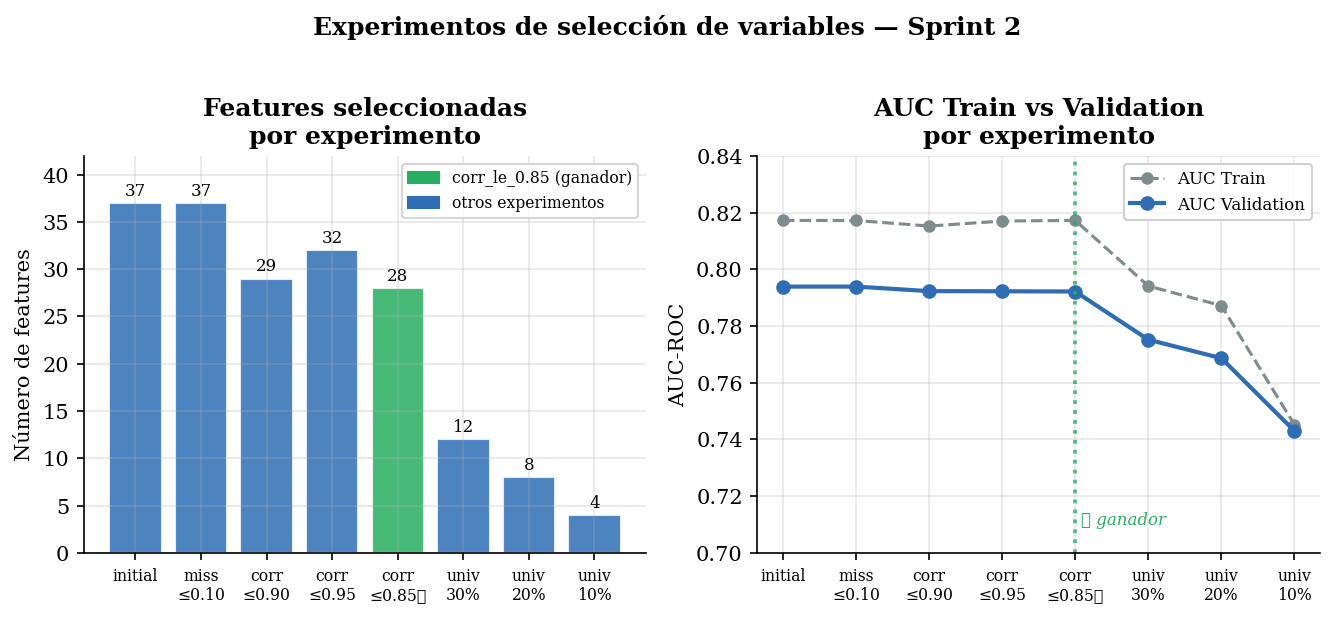
\includegraphics[width=\columnwidth]{fig_feature_selection.png}
  \caption{Comparación de experimentos de selección de variables. Panel izquierdo: número de features por experimento (verde = ganador). Panel derecho: AUC train y AUC validación; la línea discontinua vertical marca el experimento \texttt{corr\_le\_0.85}.}
  \label{fig:feature_selection}
\end{figure}

\subsection{Decisión Final: corr\_le\_0.85}
El experimento \texttt{corr\_le\_0.85} fue adoptado como set final por ofrecer el mejor equilibrio entre:
\begin{itemize}
    \item Desempeño de validación prácticamente equivalente al set \texttt{initial} (diferencia en AUC-val de solo \textbf{0.0018}).
    \item Reducción de 37 a \textbf{28 features}, eliminando colinealidad interna.
    \item Mayor parsimonia y mejor defendibilidad metodológica frente a un jurado.
\end{itemize}

Las 28 features seleccionadas cubren dimensiones operativas (\texttt{total\_orders}, \texttt{delivered\_orders}), temporales (\texttt{recency\_days}, \texttt{customer\_lifetime\_days}), de cuotas y pago, logísticas, geográficas y de categoría de producto. Ninguna de las 13 variables excluidas por leakage figura en el set final.

\section{Evaluación vs. Baseline del Sprint 1}
\subsection{Configuración de la Evaluación}
La evaluación se realizó con el mismo script (\texttt{src/models/evaluate\_model.py}), el mismo split temporal y el mismo umbral fijo P80 = 197.01 que los experimentos de selección, garantizando comparabilidad directa:
\begin{itemize}
    \item Train: 83.589 clientes (\texttt{last\_purchase < 2018-07-01})
    \item Validation: 6.230 clientes (\texttt{last\_purchase} $\geq$ 2018-07-01)
    \item Features: 28 (set \texttt{corr\_le\_0.85})
\end{itemize}

\subsection{Métricas en Validación}
La Tabla~\ref{tab:metrics} compara las métricas del Sprint 2 contra el baseline logístico del Sprint 1.

\begin{table}[h]
\centering
\caption{Comparación de Métricas: Baseline Sprint 1 vs Sprint 2}
\label{tab:metrics}
\begin{tabular}{lrrr}
\toprule
Métrica & Baseline S1 & Sprint 2 Val & Mejora \\
\midrule
Precision  & 0.3000 & 0.4766 & +58.9\% \\
Recall     & 0.1600 & 0.6294 & +293.4\% \\
F1-Score   & 0.2100 & 0.5424 & +158.3\% \\
ROC-AUC    & 0.5355 & 0.7929 & +48.1\% \\
Gini       & 0.0710 & 0.5858 & +724.4\% \\
\bottomrule
\end{tabular}
\end{table}

La Figura~\ref{fig:metrics} ilustra visualmente el contraste entre ambas versiones del modelo.

\begin{figure}[h]
  \centering
  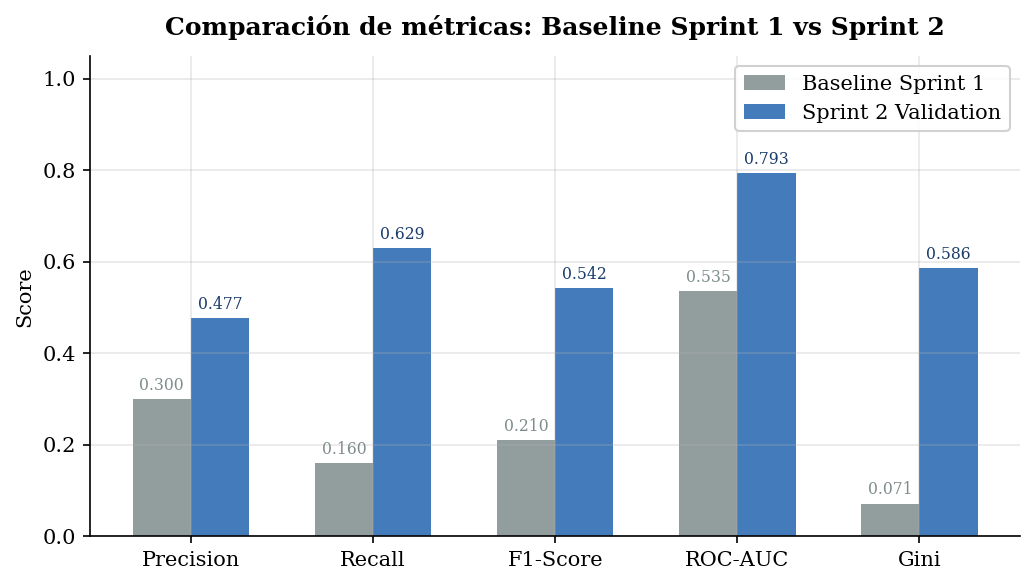
\includegraphics[width=\columnwidth]{fig_metrics_comparison.png}
  \caption{Comparación de métricas de clasificación entre el baseline de regresión logística del Sprint 1 y el modelo de Sprint 2 (\texttt{corr\_le\_0.85}, 28 features). Mejora sustancial en todas las métricas principales.}
  \label{fig:metrics}
\end{figure}

\subsection{Curva ROC y Coeficiente de Gini}
La Figura~\ref{fig:roc} presenta la curva ROC del Sprint 2 junto a la curva aproximada del baseline del Sprint 1. El área bajo la curva sube de 0.5355 a \textbf{0.7929}, y el Gini de 0.071 a \textbf{0.586}, evidenciando que el enriquecimiento de variables y el control de leakage produjeron separabilidad real.

\begin{figure}[h]
  \centering
  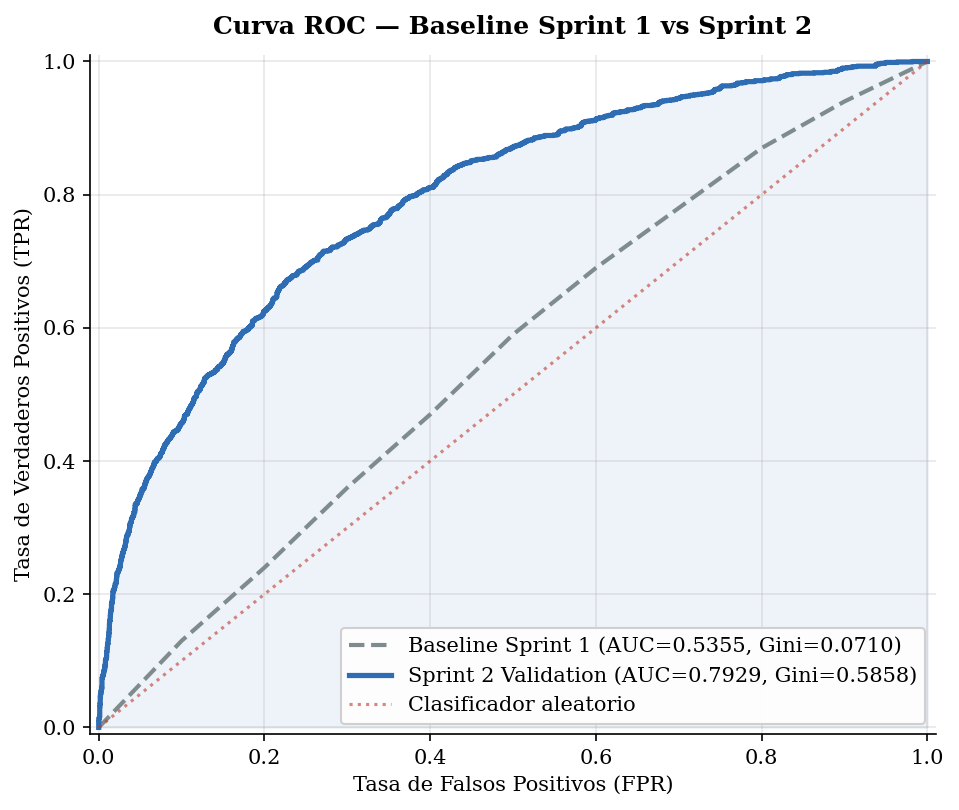
\includegraphics[width=\columnwidth]{fig_roc_sprint2.png}
  \caption{Curva ROC comparada entre el baseline del Sprint 1 (línea discontinua) y el modelo del Sprint 2 (línea continua). El área bajo la curva del Sprint 2 (AUC = 0.7929, Gini = 0.5858) supera ampliamente la diagonal aleatoria y el baseline previo (AUC = 0.5355).}
  \label{fig:roc}
\end{figure}

\subsection{Matriz de Confusión}
Sobre el conjunto de validación (6.230 clientes), el modelo produce:
\begin{equation}
\text{CM} = \begin{pmatrix} TN = 3825 & FP = 983 \\ FN = 527 & TP = 895 \end{pmatrix}
\end{equation}

El modelo identifica correctamente al \textbf{62.9\%} de los clientes premium (Recall) con una precisión del \textbf{47.7\%}. El Recall es el indicador más crítico en el contexto de negocio: detectar la mayor proporción posible del segmento de alto valor para orientar acciones de retención.

\section{KPIs de Negocio y Defensa del Target}
\subsection{KPIs Observados}
Los KPIs finales se calcularon sobre la master table limpia con el umbral fijo dev = 197.01. La Tabla~\ref{tab:kpis} resume los indicadores por segmento.

\begin{table}[h]
\centering
\caption{KPIs Segmentados — Premium vs Regular}
\label{tab:kpis}
\resizebox{\columnwidth}{!}{%
\begin{tabular}{lrr}
\toprule
KPI & Premium & Regular \\
\midrule
Clientes                     & 19.220 (20.00\%) & 76.876 (80.00\%) \\
Facturación total            & BRL 8.088.732 (56.03\%) & BRL 6.348.316 (43.97\%) \\
Ticket promedio              & BRL 402.66 & BRL 92.27 \\
Órdenes promedio             & 1.09 & 0.94 \\
Lifetime promedio (días)     & 7.26 & 1.24 \\
Máx. cuotas promedio         & 4.70 & 2.47 \\
Uso de más de 1 cuota        & 71.55\% & 42.60\% \\
Con entrega tardía           & 9.28\% & 6.93\% \\
Recency promedio (días)      & 221.16 & 227.31 \\
\bottomrule
\end{tabular}%
}
\end{table}

La Figura~\ref{fig:kpis} ilustra la concentración de facturación y la diferencia de ticket promedio entre segmentos.

\begin{figure}[h]
  \centering
  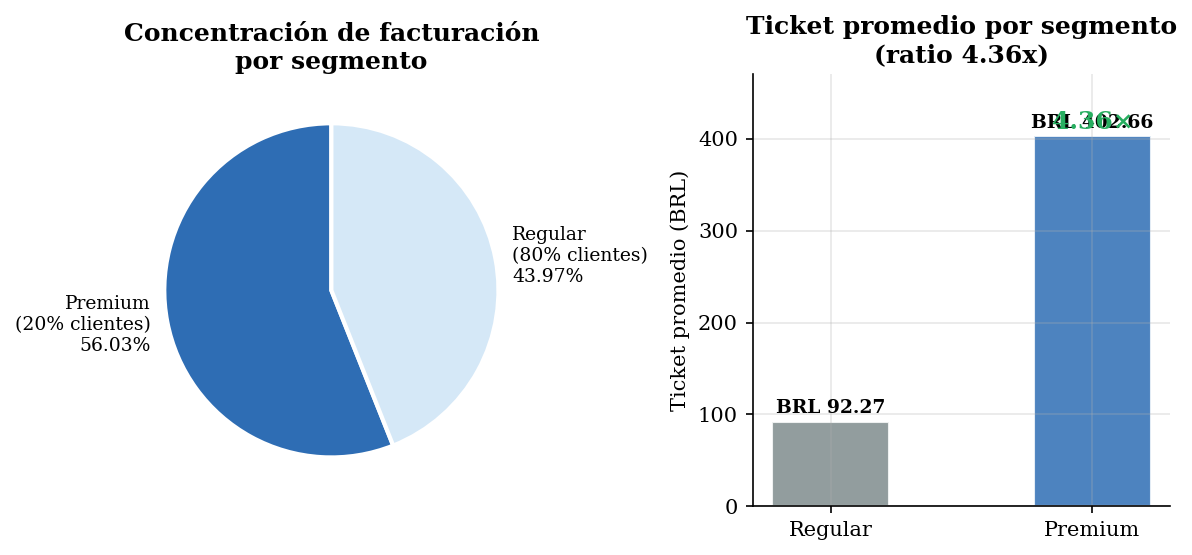
\includegraphics[width=\columnwidth]{fig_kpis_negocio.png}
  \caption{KPIs de negocio. Izquierda: concentración de facturación por segmento (el 20\% premium concentra el 56.03\% de la facturación). Derecha: ticket promedio por segmento (ratio 4.36x).}
  \label{fig:kpis}
\end{figure}

\subsection{Lectura de Negocio}
Tres observaciones justifican la validez económica del segmento:
\begin{itemize}
    \item El ratio \textbf{20\% / 56\%} indica que el target captura un segmento de valor real y no ruido estadístico.
    \item El ticket premium de BRL 402.66 es \textbf{4.36 veces} el ticket regular (BRL 92.27), coherente con la paradoja de compra única de alto valor documentada en el Sprint 1.
    \item El mayor lifetime (5.9×) y el mayor uso de cuotas (71.55\% vs 42.60\%) validan que las nuevas features del pipeline capturan patrones de comportamiento diferenciales reales del segmento premium.
\end{itemize}

\section{Conclusiones y Próximos Pasos}
\subsection{Conclusiones}
El Sprint 2 entregó los siguientes resultados verificables:
\begin{enumerate}
    \item Un \textbf{pipeline modular y reproducible} en cuatro scripts independientes, con artefactos persistidos y numerados en \texttt{data/interim/} y \texttt{data/processed/}.
    \item Un \textbf{target formalmente defendido}: P80 fijo sobre \textit{dev} = BRL 197.01, con política de umbral \texttt{fit}/\texttt{apply} y exclusión documentada de cancelaciones.
    \item \textbf{18 variables nuevas} que amplían el espacio de features más allá del RFM básico del Sprint 1.
    \item Una \textbf{selección experimental} con 8 esquemas y el set óptimo de 28 features (\texttt{corr\_le\_0.85}), libre de las 13 variables excluidas por leakage.
    \item \textbf{Mejora sustancial} en todas las métricas de clasificación: ROC-AUC 0.5355 $\to$ 0.7929 (+48.1\%), F1 0.21 $\to$ 0.54 (+158.3\%), Gini 0.071 $\to$ 0.586 (+724.4\%).
    \item \textbf{KPIs económicamente sólidos}: 20\% premium, 56\% facturación, ticket 4.36× el regular.
\end{enumerate}

\subsection{Próximos Pasos — Sprint 3}
Para el Sprint 3 se propone:
\begin{enumerate}
    \item \textbf{Ventanas temporales}: separar la ventana de observación (construcción de features) de la ventana de outcome (etiquetado de \textit{is\_premium}) para una predicción verdaderamente prospectiva.
    \item \textbf{Modelos de mayor capacidad}: evaluar Gradient Boosting y ensambles sobre las 28 features validadas.
    \item \textbf{Análisis de valor económico}: estimar el CAC máximo recomendable por cliente premium a partir del ticket promedio y la tasa de retención estimada.
    \item \textbf{Validación temporal adicional}: probar estabilidad de las features con splits de fechas distintos para confirmar robustez del pipeline.
\end{enumerate}

\begin{thebibliography}{1}

\bibitem{rfmt_methodology}
A. Ullah, M. I. Mohmand, H. Hussain, S. Johar, I. Khan, S. Ahmad, H. A. Mahmoud, and S. Huda,
``Customer Analysis Using Machine Learning-Based Classification Algorithms for Effective Segmentation Using Recency, Frequency, Monetary, and Time,''
\emph{Sensors}, vol. 23, no. 6, p. 3180, Mar. 2023. [Online]. Available: \url{https://doi.org/10.3390/s23063180}

\bibitem{random_forest}
L. Breiman,
``Random Forests,''
\emph{Machine Learning}, vol. 45, no. 1, pp. 5--32, Oct. 2001. [Online]. Available: \url{https://doi.org/10.1023/A:1010933404324}

\bibitem{gini_index}
C. Genuer, J.-M. Poggi, and C. Tuleau-Malot,
``Variable selection using random forests,''
\emph{Pattern Recognition Letters}, vol. 31, no. 14, pp. 2225--2236, Oct. 2010.

\end{thebibliography}

\end{document}
